\documentclass{tufte-book}

\usepackage{amsmath, amsthm}
\usepackage{graphicx}
\setkeys{Gin}{width=\linewidth,totalheight=\textheight,keepaspectratio}
\graphicspath{{graphics/}}

\title{STAT 244 \\ Homework 7}
\author{Joe Seidel}
\date{\today}

\usepackage{booktabs}
\usepackage{units}
\usepackage{fancyvrb}
\fvset{fontsize=\normalsize}
\usepackage{multicol}
\usepackage{lipsum}
\usepackage{pdfpages}
\usepackage{tikz}
\usepackage{wasysym}

\newcommand{\doccmd}[1]{\texttt{\textbackslash#1}}% command name -- adds backslash automatically
\newcommand{\docopt}[1]{\ensuremath{\langle}\textrm{\textit{#1}}\ensuremath{\rangle}}% optional command argument
\newcommand{\docarg}[1]{\textrm{\textit{#1}}}% (required) command argument
\newenvironment{docspec}{\begin{quote}\noindent}{\end{quote}}% command specification environment
\newcommand{\docenv}[1]{\textsf{#1}}% environment name
\newcommand{\docpkg}[1]{\texttt{#1}}% package name
\newcommand{\doccls}[1]{\texttt{#1}}% document class name
\newcommand{\docclsopt}[1]{\texttt{#1}}% document class option name
\DeclareMathOperator{\proj}{proj}
\newcommand{\vct}{\mathbf}


\newcommand{\dprod}[2]{\langle #1, #2 \rangle}
\newcommand{\Var}{\mathrm{Var}}
\newcommand{\Cov}{\mathrm{Cov}}
\newcommand{\MSE}{\mathrm{MSE}}
\newcommand{\MLE}{\mathrm{MLE}}
\newcommand{\erf}{\mathrm{erf}}

\newtheoremstyle{mytheoremstyle} % name
	{\topsep}		% Space above
	{\topsep}		% Space below
	{\itshape}		% Body font
	{}			% Indent amount
	{\bfseries}	% Theorem head font
	{\textnormal{:}}	% Punctuation after theorem head
	{.5em}		% Space after theorem head
	{}			%Theorem headspec
\theoremstyle{mytheoremstyle}
\newtheorem*{thm}{Thm.}

\newtheoremstyle{mylemstyle} % name
	{\topsep}		% Space above
	{\topsep}		% Space below
	{\itshape}		% Body font
	{}			% Indent amount
	{\bfseries}	% Theorem head font
	{\textnormal{:}}	% Punctuation after theorem head
	{.5em}		% Space after theorem head
	{}			%Theorem headspec
\theoremstyle{mylemstyle}
\newtheorem*{lem}{Lem.}


\newtheoremstyle{mydefstyle} % name
	{\topsep}		% Space above
	{\topsep}		% Space below
	{\normalfont}	% Body font
	{}			% Indent amount
	{\bfseries}	% Theorem head font
	{\textnormal{:}}	% Punctuation after theorem head
	{.5em}		% Space after theorem head
	{}			%Theorem headspec
\theoremstyle{mydefstyle}
\newtheorem*{mydef}{Def.}
\newtheorem*{ex}{E.g.}

\begin{document}

\maketitle
\pagenumbering{gobble}
\newpage
\pagenumbering{arabic}

\subsection{Question 1}
Suppose $X$ follows a geometric distribution with parameter $p$.

\begin{enumerate}

\item Derive the likelihood ratio for testing the hypothesis $p=p_0$ versus the alternative $p \neq p_0$.

\newthought{The} variable $X$ has PMF given

\[ p(X=x) = p(1-p)^{x-1} \text{ , } x=1,2,... \]

We have a composite hypothesis a generalized likelihood ratio test is in order.

\[ \Lambda = \frac{\max_{p \in w_0}[L(p)]}{\max_{p \in \Omega}[L(p)]} \]

Where the rejection region consists of small values for $\Lambda$.  In this case $w_0 = \{p_0\}$ and $\Omega = \{ 0 < p < 1\}$

\[ \max_{p \in w_0}[L(p)] = p_0(1-p_0)^{x-1}. \]

For the denomitor we have to maximize the likelihood for $p \in \Omega$.  Which is the mle of $f(x \mid p) = p(1-p)^{x}$, $\hat{p} = \frac{1}{\overline{X}}$. Which makes

\[ \max_{p \in \Omega}[L(p)] = \frac{1}{\overline{X}}\Big(1-\frac{1}{\overline{X}}\Big)^{x-1}. \]

Therefore \marginnote{It's important to note that I've set this up observing only $1$ $X$, otherwise this would look slightly different, in fact I will end up replacing $x$ for $\overline{X}$ soon.}

\[ \Lambda = \frac{p_0x(1-p_0)^{x-1}}{(1-\frac{1}{x})^{x-1}} \]

Which is the generalized likelihood ratio that will test the hypothesis.

\item For $p_0=0.01$, by some combination of numerical experimentation and mathematical analysis, find the set of possible valyes of $x$ for $X$ for which the likelihood ratio is less than $0.1$.

When graphing the the function for $\Lambda$ with $p_0=.01$, its clear that there are two values of $x$ that make likelihood ration less than $.1$.

\begin{figure}
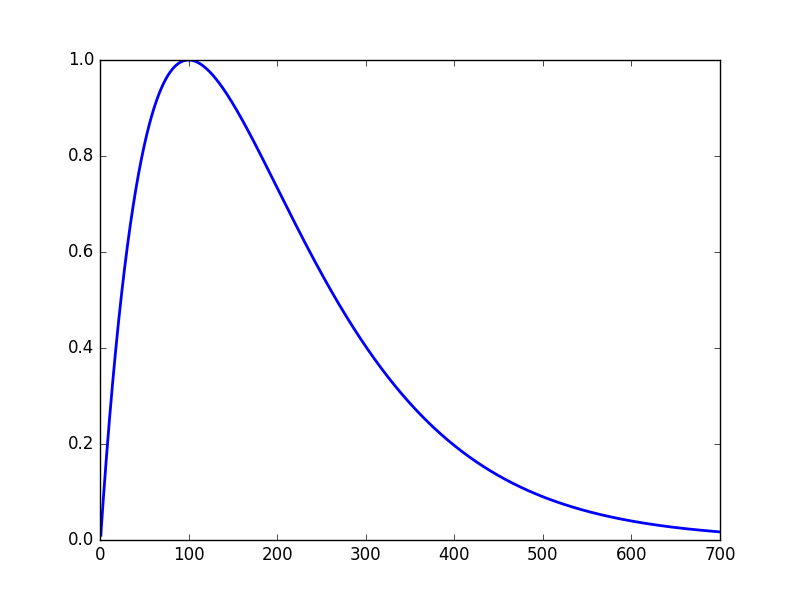
\includegraphics{q1}
\caption{The likelihood function when $p_0=.01$}
\end{figure}

I used a computer to find the values.  Since $x \in \mathbb{N}$, $x \leq 4$ and $x \geq 488$.

Hence for $x \leq 4$ we have likelihood ratio less than $0.1$.

\item Find the probability of Type 1 error for the test the rejects $p_0=0.01$ when the likelihood ratio is less than $0.1$.  Find the power of this test when $p=0.5$.  Find the power of ths test when $p=0.001$.

\newthought{To find} $\alpha$ given $\Lambda \leq .1$ and $H_0$:$p=.01$ take
\begin{align*}
\alpha &= P(x \leq 4 \mid p=.01) + P(x \geq 488 \mid p=.01)\\
&= \sum_{i=1}^4P(x=i \mid p=.01) + 1 - P(x \leq 488 \mid p=.01)\\
&= .04 + .007\\
&= .047
\end{align*}

Next I need to find the the power f the test when $p=.5$ and $p=.0001$.\marginnote{Per Reintiz's office hours, this is to say, type two error given these alternative values for $p$.}

Recall, $\pi = P(H_1 \mid H_1)$.

When $p=.5$
\begin{align*}
\pi &= P(H_1 \mid H_1)\\
&= P(x \leq 4 \cup x \geq 488 \mid p=.5)\\
&= \sum_{i=1}^4P(x=i \mid p=.5) + 1 - P(x \leq 488 \mid p=.5)\\
&= .9375
\end{align*}

When $p=.001$
\begin{align*}
\pi &= P(H_1 \mid H_1)\\
&= P(x \leq 4 \cup x \geq 488 \mid p=.001)\\
&= \sum_{i=1}^4P(x=i \mid p=.001) + 1 - P(x \leq 488 \mid p=.001)\\
&= .62
\end{align*}
\end{enumerate}


\subsection{Question 2 Rice 9.12}

Let $X_1,...,X_n$ be a random sample from an exponential distribution with the density function $f(x\mid \theta)= \theta e^{-\theta x}$.  Derive a likelihood ratio test of $H_0$: $\theta = \theta_0$ versus $H_A$: $\theta \neq \theta_0$, and show that the rejection region is of the form $\{\overline{X}e^{-\theta_0\overline{X}} \leq c \}$.

\newthought{First}, \marginnote{I've found this in previous homeworks.} recall that the mle of $L(\theta)$ is $\hat{\theta}=\frac{1}{\overline{X}}$.  Set up the likelihood ratio test

\[ \Lambda = \frac{\max_{p \in w_0}[L(p)]}{\max_{p \in \Omega}[L(p)]}. \]

The numerator will be

\[ L(\theta_0) = \prod_{i=1}^n \theta e^{-\theta_0 x_i} \]
and the denomitaor

\[ L(\hat{\theta}) = \prod_{i=1}^n \frac{1}{\overline{X}} e^{-\frac{x_i}{\overline{X}}}. \]

Then
\begin{align*}
\Lambda &= \frac{\prod_{i=1}^n \theta e^{-\theta_0 x_i}}{\prod_{i=1}^n \frac{1}{\overline{X}} e^{-\frac{x_i}{\overline{X}}}}\\
&= \frac{\theta_0^n e^{-\theta_0 n\overline{X}}}{\frac{1}{\overline{X}^n}e^{-\frac{\overline{X}n}{\overline{X}}}}\\
&= \frac{\theta_0^n \overline{X}^n e^{-\theta_0 n\overline{X}}}{e^{-n}}\\
&= \big(e \theta_0 \overline{X} e^{(-\theta_0 \overline{X})}\big)^n
\end{align*}

Where $H_0$ is rejected when $\Lambda$ is small.  Since $e, n, \theta$ are positive, $\Lambda$ is small when $\overline{X} e^{(-\theta_0 \overline{X})}$ is small.

\begin{align*}
\big(e \theta_0 \overline{X} e^{(-\theta_0 \overline{X})}\big)^n < c_1\\
e \theta_0 \overline{X} e^{(-\theta_0 \overline{X})} < c_1^{\frac{1}{n}}\\
\overline{X} e^{(-\theta_0 \overline{X})} < \frac{c_1^{\frac{1}{n}}}{\theta_0 e}\\
\end{align*}

Therefore, we see the rejection region takes the form $\overline{X} e^{(-\theta_0 \overline{X})} \leq c =\frac{c_1^{\frac{1}{n}}}{\theta_0 e}$.

\subsection{Question 3 Rice 9.13}
Suppose, to be specific, that in problem 12, $\theta_0=1$, $n=10$, and that $\alpha=.05$.  In order to use the test, we must find the appropriate value of $c$.
\begin{enumerate}

\item Show that rejection region is of the form $\{\overline{X} \leq x_0\} \cup \{ \overline{X} \geq x_1 \}$, where $x_0$ and $x_1$ are deterimined by $c$.

\newthought{Now} that we are given a value for $\theta_0$ we have

\[ f(x\mid \theta_0) = xe^{-x}. \]

But we also found in the previous question that our test rejects when
\[ f(\overline{X} \mid \theta_0) = \overline{X} e^{(-\overline{X})} \]
is small, specifically when less than $c$.  To see why it takes the form
$\{\overline{X} \leq x_0\} \cup \{ \overline{X} \geq x_1 \}$, consider the graph of the function.

\begin{figure}
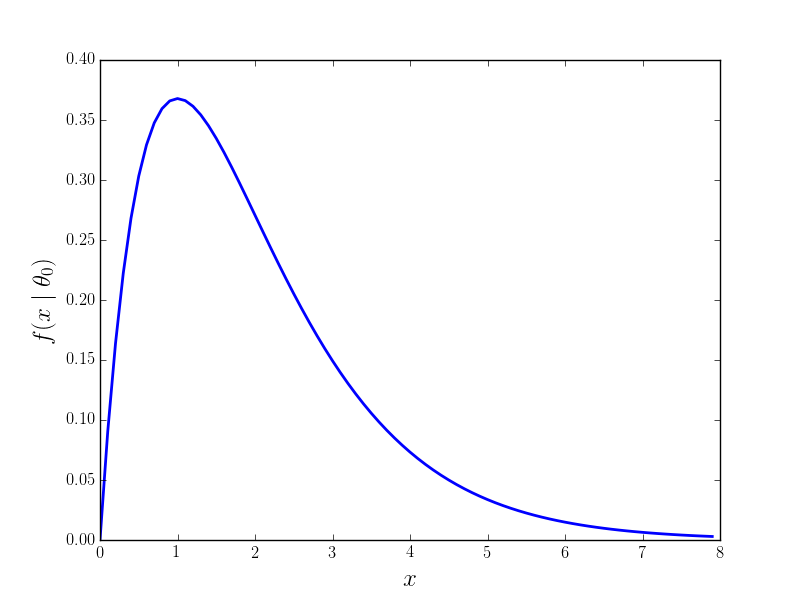
\includegraphics{q3}
\caption{}
\end{figure}

There would be a $c$ chosen that corresponds with the $Y$ axis of the graph and a horizontal line would interect the function at two values of $x$.

\item Explain why $c$ should be chosen so that $P(\overline{X} e^{(-\overline{X})} \leq c) = .05$.

\newthought{This} is just a restatement of Type I error under Neyman-Pearson.

\[Pr(\text{Reject }H_0 \mid H_0) = Pr(x \in [0, c] \mid \theta_0) \]

Which can be worded to say, the probability that $x$ falls in the rejection zone.  Furthermore, we found that $P(\overline{X} e^{(-\overline{X})})$ provides a rejection zone for $\Lambda$.  What remains is to determine how willing we are to make Type 1 error.

If we want $\alpha=.05$ then we should set
\[ Pr(x \in [0, c] \mid \theta_0) = Pr(f(\overline{X} \mid \theta)) < c) = .05 \]

to determine what $c$ should be.

\item Explain why $\sum_{i=1}^10 X_i$ and hence $\overline{X}$ follow gamma distributions when $\theta_0=1$.  How could this knowledge be used to choose c?

Under $H_0$: $\theta_0=1$ $X_i \sim Exponetial(1)$ which is a special ase of $\Gamma(1,\lambda)$ or in this particular case $\Gamma(1,1)$.  On the last homework, I found that $\sum_{i=1}^n X_i \sim \Gamma(n,1)$ and $\overline{X} \sim \Gamma(n,n)$.  Knowing the exact distribution, means I could compute the exact value of $c$ for which $95$ coverage for acceptable values of $H_0$.

In this day and age, a computer would be the easiest way to do this.  The gist would be first solve $f(\overline{X})=c$ to get $x_0(c)$ and $x_1(c)$.  Then solve
\[ \alpha(c) = F(x_0(c)) + 1-F(x_1(c)) \]

Where $F(x)$ is cdf of $\Gamma(10,10)$.

\item Suppose you hadn't thought of the preceding fact.  Explain how you could determine a good approximation to $c$ by generating random numbers on a computer (simulation).

\newthought{Generate} a bunch of samples from $Exponential(1)$ of size $n=10$.  Then compute $\overline{X}e^{\overline{X}}$ for each sample. Sort the result and set the cuttoff as the value indexed at the $5\%$ of the number of samples generated.  For example, if the results are stored in some list of size $10000$ then you'd take value indexed at list[500] as the cuttoff value for a close approximation.
\end{enumerate}

\subsection{Question 4}

Call "This, it thus, and" Class I workds; Class II is "everything else".   For each of 215 groups of 5 of James Mill's sentences, the number of Class I words was counted.

Test whether a Binomial Distribution $(n=5, \theta)$ fits these data.

\begin{marginfigure}
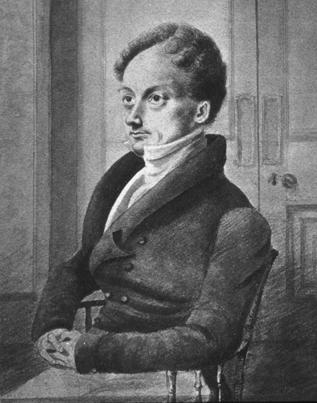
\includegraphics{James_Mill}
\caption{James Mill, the economist.  Apparently, this guy spent his life in love with a woman who had already been promised to another.  After years of her marriage, the husband died.  The two finally got together.  Then Like 6 months passed and she died.  Bummer, right?}
\end{marginfigure}

\newthought{First}, knowing the MLE of a binomial will be useful.

\begin{align*}
L(\theta) &= \prod_{i=1}^n \binom{n}{x_i} \theta^{x_i}(1-\theta)^{n-x_i} \\
&= \prod_{i=1}^n \binom{n}{x_i} \theta^{\sum_{i=1}^n x_i}(1-\theta)^{n- \sum_{i=1}^n x_i}\\
\end{align*}

Taking the log and the derivative we have

\[ \frac{d}{d\theta} \log L(\theta) = \frac{\overline{X}n}{\theta} + \frac{n- \overline{X}n}{\theta - 1} \]

Setting the above equal to zero and solving for $\theta$ give the mle.

\[ \hat{\theta} = \overline{X} \]

Using the table we can compute the mle, $\hat{\theta} = 339/215(5) = .31$.  With this a few rows can be added to the table.

Expected is calculated

\[ E_i = \binom{n}{x_i} \hat{\theta}^x_i (1-\hat{\theta})^{n-x_i} \cdot 225 \text{ for } x_i = 0,1,2,..,n=5 \]

Then calculate each component of

\[ X^2 = \sum_{i=1}^m \frac{[x_i - np_i(\hat{\theta})]^2}{np_i(\hat{\theta})}\]

Where $m=6$ cells.

\begin{table}
\centering
\begin{tabular}{l|llllll}
No. Class I words & 0 & 1 & 2 & 3 & 4 & 5 \\
No. groups(observed) & 87 & 11 & 51 & 42 & 20 & 4 \\
No. groups(expected) &34&76&68&30&7&1\\
Component of Chi-Squared &82.62&55.59&4.25&4.8&24.14&9.0
\end{tabular}
\caption{Class I words}
\label{millwords}
\end{table}

Summing up the last row of the table, the chi-square statistic $X^2=180.4$ with 4 degrees of freedom (6 cells and one parameter was estimated from the data).  Finally, our rejection region is $X^2 > \chi_4^2(\alpha)$.  If we specify $\alpha=.005$ (giving our null hypothesis the best chance) our test is

\[ 180.4 = X^2 > \chi_4^2(.005) = 14.86 \]

Which rejects the null hypothesis that $X \sim Bin(n=5, \theta)$.


\subsection{Question 5}
The members of a community are classified by Blood type:

\begin{table}
\centering
\begin{tabular}{llllll}
O&A&B&BA&Total\\
121&120&79&33&353
\end{tabular}
\caption{Community blood types}
\label{bloodtypes}
\end{table}

Theory has is that the probabilities of those types depends on gene frequency parameters $r,p,q$, where $r+p+q=1$ and $P($"O"$)=r^2$, $P($"A"$)=p^2+2pr$, $P($"B"$)=q^2+2qr$, and $P($"AB"$)=2pq$.  Using numerical methods (that is, a method such as that described in Chapter 5 of Stigler's notes) we can find the MLEs of $r,p,q$; they are
\begin{align*}
\hat{r} &= 0.580 \\
\hat{p} &= 0.246 \\
\hat{q} &= 0.173 \\
\end{align*}

Test if the community fits the theory. \marginnote{Can't afford to estimate three parameters with only 4 cells!}

\newthought{Since} there are only 4 cells, I cannot afford to estimate all 3 parameters.  Instead, I'll just estimate 2 and the substute the third $r'= 1- .246 -.173 = .581$



\begin{table}
\centering
\caption{Blood Types with Chi-Square}
\label{blod2}
\begin{tabular}{l|lllll}
                   & O      & A      & B    & BA   & Total  \\ \cline{2-6}
observed           & 121    & 120    & 79   & 33   & 353    \\
expected           & 119.15 & 122.26 & 81.5 & 30.5 & 353.41 \\
Comp of Chi-Square &0.02&0.04&0.08&0.2&.342\\
\end{tabular}
\end{table}

The table above was completed using similiar methods described in the previous question.  The chi-squared statistic is $X^2 = .342$.  We have 1 degree of freedom ($4-1-2 = 1$).  Choose $\alpha=.1$, then

\[ .342 = X^2 < \chi_1^2(.1) = 2.71 \]

Which supports the null that the community fits the theory.


\subsection{Question 6}
Are finger print patterns genetic, or are the developmental?  In 1892\marginnote{Columbus sailed the ocean blue...or was it 1492?}, Francis Galton compiled the following table on the relationship between the patterns on the same finger of 105 sibling pairs.  Test the hypothesis that the patterns are independent for example, that knowing one sibiling (A) has Whorl on the finger does not help in predicting the pattern of the other (B).

\begin{table}
\centering
\caption{Galton's Siblings}
\label{galton}
\begin{tabular}{l|lll|l}
           & \multicolumn{3}{l}{A Children}                                    &        \\
B Children & \multicolumn{1}{l|}{Arches} & \multicolumn{1}{l|}{Loops} & Whorls & Totals \\ \hline
Arches     & \multicolumn{1}{l|}{5}      & \multicolumn{1}{l|}{12}    & 2      & 19     \\ \hline
Loops      & \multicolumn{1}{l|}{4}      & \multicolumn{1}{l|}{42}    & 15     & 61     \\ \hline
Whorls     & \multicolumn{1}{l|}{1}      & \multicolumn{1}{l|}{14}    & 10     & 25     \\ \hline
Totals     & \multicolumn{1}{l|}{10}     & \multicolumn{1}{l|}{68}    & 27     & 105    \\ \hline
\end{tabular}
\end{table}

\newthought{Calculate} $\chi^2$ squared statistic

\[ \chi^2 = \sum_{i=1}^3 \sum_{j=1}^3 \frac{\Big[X_{ij} - \Big(\frac{X_{i+}X_{+j}}{n}\Big)\Big]^2}{\Big(\frac{X_{i+}X_{+j}}{n}\Big)} \]

Which computes to $\chi^2 = 11.16$.  We check this value with the table, given $(r-1)(c-1)=2\cdot 2=4$ degress of freedom.  From the Chi-Squared table, we'd have a p-value $<.025$ which \marginnote{Small p-values provide strong evidence against Null when chi-square testing.}provides fairly strong evidence against the null hypothesis that the patterns are independent.


\subsection{Question 7}
For the Bortkiewicz Death by Horsekick Data, test the hypothesis that the data follow a Poisson distribution.  You should group the count for "4 or more" a one category.

\newthought{First}, estimate $\lambda$.  The likelihood function is
\begin{align*}
L(\lambda) &= \prod_{i=1}^n e^{-\lambda} \frac{\lambda^{x_i}}{x_i!} \\
&= e^{-n\lambda} \lambda^{\overline{X}n} \prod_{i=1}^n \frac{1}{x_i!}\\
\end{align*}
Then take the $\log L(\lambda)$
\[ \log L(\lambda) = -n\lambda + \overline{X}n \log(\lambda) + \log(\prod_{i=1}^n \frac{1}{x_i!})\]

Next, differentiate
\[ \frac{d \log L(\lambda)}{d \lambda} = -n + \frac{\overline{X}n}{\lambda} \]

Then, \marginnote{If this was a problem about MLE, I'd take second derivative to show this maximizes.  I did this in previous homeworks so I'm not doing it here.  An important step to remember, none-the-less.}by setting the above equal to $0$, solve for $\lambda$ to get
\[ \hat{\lambda} = \overline{X} \]

To test the hypothesis, we'll create a $X^2$ statistic using expected and compaired values.  To find expected values, compute $\hat{\theta}$ given the data.

\[ \hat{\theta} = \frac{0 \cdot 144 + 1 \cdot 99 + 2 \cdot 32 + 3 \cdot 11 + 4 \cdot 2}{280} = .7 \]

\begin{table}
\centering
\caption{Horse Kicks}
\label{bort}
\begin{tabular}{l|lllll}
No. Deaths       & 0   & 1  & 2  & 3  & $\geq$ 4 \\
Observed         & 144 & 91 & 32 & 11 & 2        \\
Expected         &139.04&97.33&34.07&7.95&1.61     \\
Comp Chi-Squared &0.18&0.41&0.13&1.17&0.10
\end{tabular}
\end{table}

From the table we have chi-squared statistic $X^2=1.98$.  With $k=5-1-1=3$ degress of freedom, $\chi_3^4(.1) = 6.25$.

\[ X^2 = 1.98 < \chi_3^4(.1) = 6.25 \]

The value $X^2$ is even less than the expected value $k=3$.  Additionally, looking at the Chi-Square table we confirm that the p-value is greater than .1 and we accept the null hypothesis that the data follow Poisson distribution.
\end{document}
\grid
